\documentclass[15pt,journal]{IEEEtran}

\usepackage{algorithm}
\usepackage{algpseudocode}
\usepackage{hyperref}
\hypersetup{
    colorlinks=true,
    linkcolor=blue,
    filecolor=magenta,      
    urlcolor=blue,
    pdftitle={Overleaf Example},
    pdfpagemode=FullScreen,
    }
\usepackage[style=ieee]{biblatex}
\usepackage{amsmath,bm}
\usepackage{cite}
\usepackage{url}
% \hyphenation{op-tical net-works semi-conduc-tor}
\usepackage{graphicx}  %needed to include png, eps figures
\usepackage{float}  % used to fix location of images i.e.\begin{figure}[H]

\begin{document}

% paper title
\title{\LARGE{ \textbf{ Indian Institute of Information Technology Vadodara(IIITV)}}\\ \LARGE{CS362 Artificial Intelligence Laboratory Report}}



\author{\Large{
\IEEEauthorblockN{$^{1}$ Ade Eshwar Nayak(202051009) \\$^{2}$ Ankit Kumar Mishra(202051028)\\ $^{3}$ Ghiya Jay Manishbhai(202051073) \\$^{4}$ Hariom Kaushal(202051080) }
}%
}




% make the title area
\maketitle

% As a general rule, do not put math, special symbols or citations
% in the abstract or keywords.
\section{\large{\underline{Introduction}}}
In this lab report, we will present four chosen experiments and provide an overview of each experiment, along with our observations and the results that we obtained. All four experiments are: 
\begin{itemize}
    \item \textbf{Week0}: To be able to model a given problem in terms of state space search problem and solve the same using BFS/ DFS.
    \item \textbf{Week1}: Learning Objective: To design a graph search agent and understand the use of a hash table, queue in state space search.
    \item \textbf{Week2} : To understand the use of Heuristic function for reducing the size of the search space.  Explore non-classical search algorithms for large problems.
    \item \textbf{Week5}: Game Playing Agent | Minimax | Alpha-Beta Pruning
    \item \textbf{Week6}: Understand the graphical models for inference under uncertainty, build Bayesian Network in R, Learn the structure and CPTs from Data, naive Bayes classification with dependency between features.  
\end{itemize}
For these Experiment we have used google colab interface and a Github repository link is also provided for the code reference.
\section{\large{\underline{WEEK 0}}}
To be able to model a given problem in terms of state space search problem and solve the same using BFS/ DFS
\subsection{In the rabbit leap problem, three east-bound rabbits stand in a line blocked by three west-bound rabbits. They are crossing a stream with stones placed in the east west direction in a line. There is one empty stone between them. The rabbits can only move forward one or two steps. They can jump over one rabbit if the need arises, but not more than that. Are they smart enough to cross each other without having to step into the water? 
}
\begin{figure}[H]%[!ht]
\begin {center}
\href{https://www.slideshare.net/KrishnaMadala1/ch-2-state-space-search-slides-part-1pdf}
{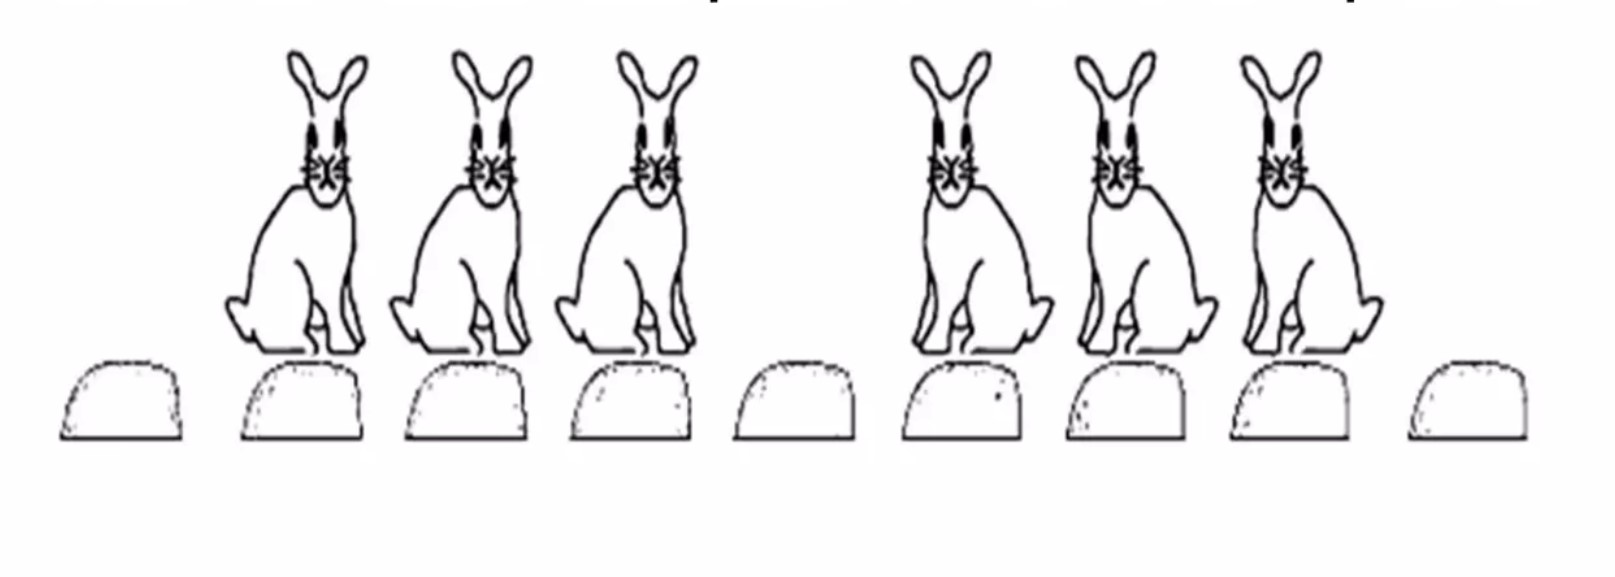
\includegraphics[width=0.48\textwidth]{image/Rabbit.jpg}}
\caption{ \cite{krishna}Rabbit Leap Problem Slide 82} % Caption change
\label{fig:ecg}
\end {center}
\end{figure}
\subsubsection{\large{Methodology}\\}
We first identified the initial state of the problem, where three east-bound rabbits are blocked by three west-bound rabbits with an empty stone in between. The goal state was the arrangement of rabbits and stones where all three east-bound rabbits had successfully crossed to the other side.

We formulated the problem as a state space search problem, where the state space was defined as the possible arrangements of rabbits and stones on the stream. The initial state was the starting arrangement of rabbits and stones, and the goal state was the arrangement where all east-bound rabbits had crossed to the other side.

The operators were defined as the actions that could be taken to move from one state to another, which included moving a rabbit one or two steps forward, jumping over one rabbit, and moving an empty stone one or two steps.

We implemented this problem in Python using BFS and DFS algorithms. For both algorithms, we defined the initial and goal states and the operator to move forward. We then implemented the BFS and DFS functions to traverse the state space graph and find a solution.

The BFS function starts with the initial state and performs a Breadth-First Search until it finds the goal state or exhausts the search space. We used a queue data structure to keep track of the states to be visited and a set to keep track of the visited states. At each iteration, we removed the next state from the queue and checked if it was the goal state. If not, we generated the child states using the move forward function and added them to the queue if they were not already visited. We also kept track of the nodes evaluated and the time taken to find the solution.

The DFS function works in a similar way as the BFS function, but instead of a queue, it uses a stack to keep track of the states to be visited. It also keeps track of the path taken to reach each state. The DFS function performs a Depth-First Search until it finds the goal state or exhausts the search space. We also kept track of the nodes evaluated and the time taken to find the solution.\\
\subsubsection{\large{Result}\\}
We tested both BFS and DFS algorithms on the Rabbit Leap problem using the same initial and goal states. The initial state was ("W", "W", "W", "-", "E", "E", "E"), and the goal state was ("E", "E", "E", "-", "W", "W", "W").

The BFS algorithm found the solution in 0.0084 seconds with 752 nodes evaluated. The DFS algorithm found the solution in 0.0092 seconds with 8 nodes evaluated.\\
\subsubsection{\large{Conclusion}\\}
The Rabbit Leap problem can be solved using both BFS and DFS algorithms. However, the BFS algorithm is more efficient in terms of the number of nodes evaluated, while the DFS algorithm is faster in finding the solution. The choice of algorithm depends on the problem's specific constraints and requirements.
\subsection{The missionaries and cannibals problem is usually stated as follows. Three missionaries and three cannibals are on one side of a river, along with a boat that can hold one or two people. Find a way to get everyone to the other side without ever leaving a group of missionaries in one place outnumbered by the cannibals in that place. This problem is famous in AI because it was the subject of the first paper that approached problem-formulation from an analytical viewpoint. 
}

\begin{figure}[H]%[!ht]
\begin {center}\href{https://courses.grainger.illinois.edu/cs440/fa2019/Lectures/search-figs/missionaries.png}{
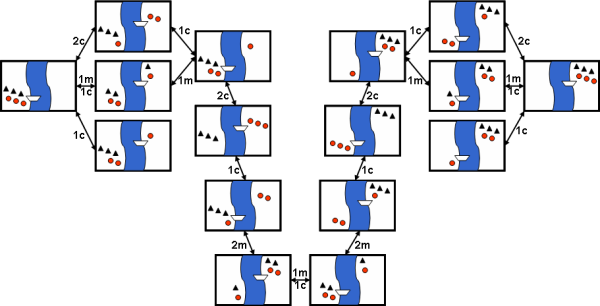
\includegraphics[width=0.48\textwidth]{image/missionaries.png}}
\caption{\cite{missionaries}The missionaries and cannibals problem} % Caption change
\label{fig:ecg}
\end {center}
\end{figure}


\begin{itemize}
\item State space: A state in the problem is defined by the number of missionaries and cannibals on each side of the river, as well as the location of the boat.
\item Initial state: The initial state of the problem is (3, 3, 1), meaning that there are three missionaries and three cannibals on the left side of the river, and the boat is on the left side.
\item Goal state: The goal state of the problem is (0, 0, 0), meaning that there are no missionaries or cannibals on the left side of the river and the boat is on the right side.
\item Operators: The operators in this problem are crossing the river with either one or two people, as long as the number of missionaries does not fall below the number of cannibals on either side of the river.
\end{itemize}

To model this problem, we can use a graph representation where each node represents a state and each edge represents a valid action. We can use either Breadth-First Search (BFS) or Depth-First Search (DFS) algorithm to traverse the graph and find the path from the initial state to the goal state.

\subsubsection{Solution using BFS}
\par We can use the BFS algorithm to solve this problem by exploring all possible states starting from the initial state in a breadth-first manner until we reach the goal state. We keep track of the visited states to avoid revisiting them, and we use a queue to keep track of the states to be explored next. The algorithm stops when the goal state is reached, and the path from the initial state to the goal state is found.

\subsubsection{Solution using DFS}
We can use the DFS algorithm to solve this problem by exploring all possible states starting from the initial state in a depth-first manner until we reach the goal state. We keep track of the visited states to avoid revisiting them, and we use a stack to keep track of the states to be explored next. The algorithm stops when the goal state is reached, and the path from the initial state to the goal state is found.

\subsubsection{Comparing BFS and DFS solutions}
Both BFS and DFS algorithms can find a solution to the Missionaries and Cannibals problem. However, BFS guarantees finding the shortest path from the initial state to the goal state, while DFS may find a longer path. In terms of time complexity, BFS may take longer since it explores all possible states in a breadth-first manner, while DFS may find a solution faster by exploring the paths in a depth-first manner.

\subsubsection{Conclusion}
The Missionaries and Cannibals problem is an interesting problem that requires finding a sequence of actions to reach the goal state while satisfying the given constraints. The state-space search problem can be modeled as a graph, and BFS and DFS algorithms can be used to find the solution. In general, BFS guarantees finding the shortest path, while DFS may find a solution faster. However, the choice of algorithm depends on the problem's size and complexity.

\section{\large{\underline{WEEK 1}}}
 To design a graph search agent and understand the use of a hash table, queue in state space search.
 
\subsection{Write a pseudocode for a graph search agent. Represent the agent in the form of a flow chart. Clearly mention all the implementation details with reasons}

\underline{Answer:}\\
\begin{algorithm}
\State Set environment for search by initializing start state, Goal state,hash set for visited nodes and Frontier queue
\State Initialize with the initial values of root = start state,cost =0,parents=null,visited [] = []
\While{Frontier is not empty }
    \State pop a element from frontier
    \State Mark it as visited 
    \If{CurrentNode.state =  Goalstate}
        \State Goal state reached
    \Else
        \State mark this state as visited node in vistied set.
    \State $possible state \gets current state$
    \For{every state}
        \If{state not visited}
            \If{state present in frontier}
                \If{ new cost $<$ previous cost}
                     \State Update the cost, parent
                \EndIf
            \Else
                \State create newNode  = currentNode
                \State cost = currentNode.cost+cost to reach currentnode to newNode
                \State parent = currentNode
            \EndIf
            \State If Goal not found, path not found
        \EndIf
    \EndFor
    \EndIf           
\EndWhile
\\
\end{algorithm}
\begin{figure}[H]%[!ht]
\begin {center}
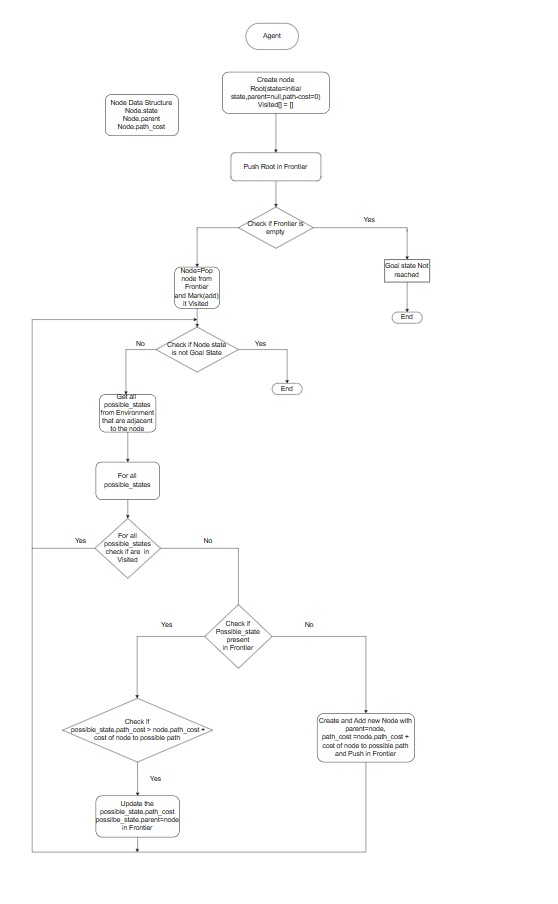
\includegraphics[height=0.40\textheight,width=0.55\textwidth]{image/flowchart.jpeg}
\caption{Flow Chart of graph search agent}
\label{fig:ecg}
\end {center}
\end{figure}

\subsection{Write a collection of functions imitating the environment for 8-Puzzle.}

\underline{Answer:}\\
The \cite{uninformed}8-puzzle is a problem consists of a 3x3 grid with eight numbered tiles and one blank space. The goal of the problem is to reach a state in which the tiles are arranged as  [[0,1,2][3,4,5][6,7,8]].
It can use  breadth-first search, depth-first search, iterative deepening search, and A* search for finding goal state.\\
Environment provides the agent with information about the current state of the problem, including the location of the tiles and the position of the blank space,legal moves that the agent can make, and provides feedback to the agent in the form of a reward or penalty based on the agent's actions.\\ 
\emph{Function}\\
{\bf{getposition()}}: return the current state(number position on board) \\
{\bf{check()}}: If the current state is goal state\\
{\bf{validate()}}: check if it is possible to move furthur or not\\
{\bf{getaction()}}: returns a list of legal actions that can be made\\
{\bf{makeaction()}}: apply action and return new state 

\begin{figure}[H]%[!ht]
\begin {center}
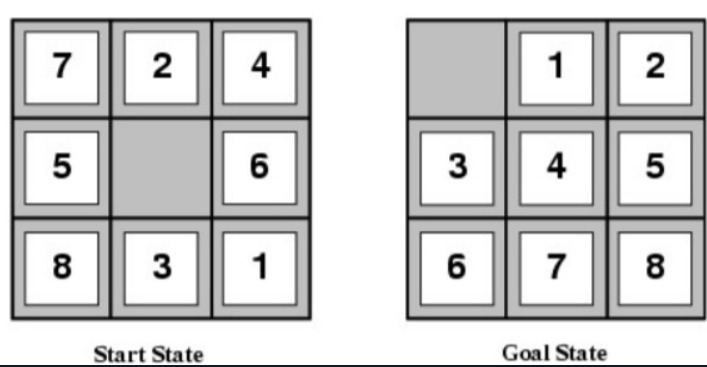
\includegraphics[width=0.48\textwidth]{image/8puzzle.jpeg}
\caption{Start and Goal state of 8-puzzle} 
\label{fig:ecg}
\end {center}
\end{figure}


\subsection{Describe what is Iterative Deepening Search ?}

\underline{Answer:}
Iterative Deepenig Search Algorithm\cite{uninformed} is used with DFS,finding the best depth limit. It does depth first search with increasing limit - 0,1,2, and so on until find the goal. It combines benefits of both DFS and BFS. It does DFS until limit depth(same as that of BFS).In every cycle, bound limit increased by one.In BFS, we store previously visited nodes and then increase the limit by 1, but here we do repeating the previous layer, for saving the memory at cost of multiple times. Therefore, memory requirements grow linearly with depth but the time complexity is same as DFS.\\ 
The time complexity of iterative deepening is same as dfs i.e. {\bf{O(b{{$\bm{^{d}}$)}}}}.  The space complexity is {\bf{O(bd)}}.
where b is the branching factor and d is the depth .


\begin{figure}[H]%[!ht]
\begin {center}
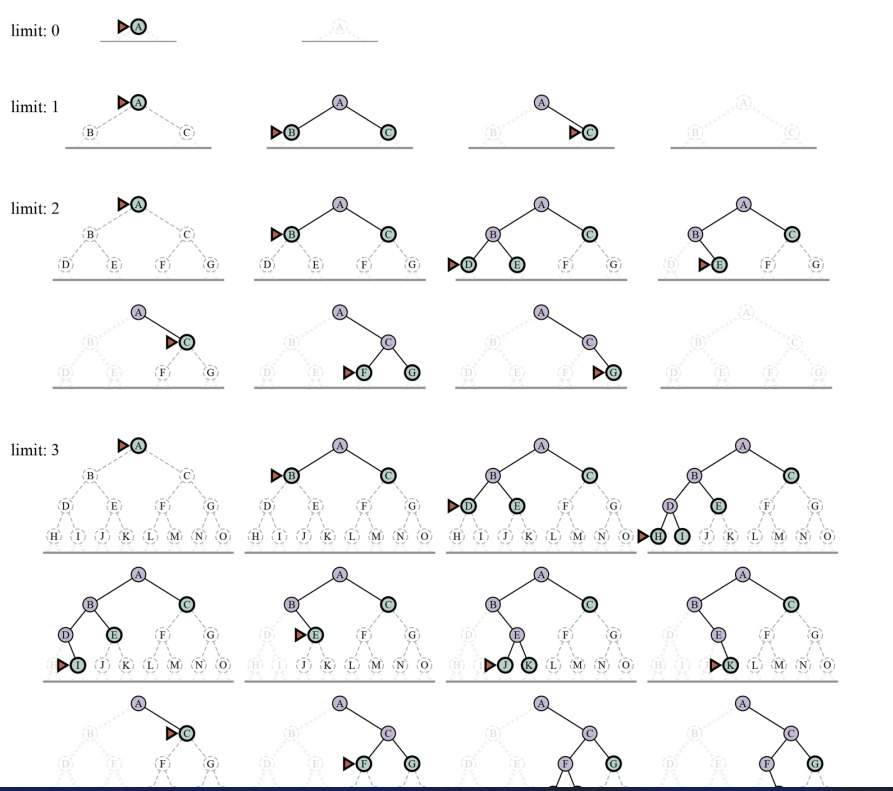
\includegraphics[width=0.48\textwidth]{image/ids.jpeg}
\caption{Iterative Deepening Search} 
\label{fig:ecg}
\end {center}
\end{figure}


\subsection{Considering the cost associated with every move to be the same (uniform cost), write a function which can backtrack and produce the path taken to reach the goal state from the source/ initial state}

\underline{Answer:}

Let cost for moving from one node to another be 1.Then the cost  at depth d is d in search graph.For path to reach goal state from source, so add nodes in visited path.Start from goal state and check from which have reached goal state.Add that node in path and do same for all.


\subsection{Generate Puzzle-8 instances with the goal state at depth “d”.}

\underline{Answer:}

For generating puzzle 8 instances with goal state at depth "d". We have to explore each and every possible states from initial state to reach the goal state.At depth d, there are bd nodes.

\subsection{Prepare a table indicating the memory and time requirements to solve Puzzle-8 instances (depth “d”) using your graph search agent.}

The space requirement for iterative deepening search agent is O(bd)\\
The time requirement for iterative deepening search agent is O(b$^d$)\\
b - branch factor\\
d - depth factor\\
So time will be exponential for this and the space will go linearly.\\

\section{\large{\underline{WEEK 2}}}
 To understand the use of Heuristic function for reducing the size of the search space.  Explore non-classical search algorithms for large problems.
\subsection{Read about the game of marble solitaire. Figure shows the initial board configuration. The goal is to reach the board configuration where only one marble is left at the centre. To solve marble solitaire, (1) Implement priority queue based search considering path cost, (2) suggest two different heuristic functions with justification, (3) Implement best first search algorithm, (4) Implement A*, (5) Compare the results of various search algorithms. 
}

\subsubsection{\Large{\textbf{Answer}}\\}
Marble solitaire requires the player to remove marbles off the board by leaping over them with other marbles until there are no more hops left. The objective is to remove as many marbles off the board as you can until there is just one marble remaining in the centre. We can treat the issue as a search problem, where the goal state is a board with only one marble remaining in the middle and the actions are moves that remove one marble by jumping over another marble, in order to solve marble solitaire using search algorithms. \\
\vspace{2mm}
\textbf{\textit{Priority queue based search considering path cost:}} \\
We can identify the shortest path to the goal state based on the cost of the path by using a priority queue-based search algorithm, such as Uniform Cost Search or A*. The number of movements necessary to get to the goal state can be thought of as the path's cost. Nodes are enlarged by the search algorithm according to their path costs, with nodes with lower path costs expanding first.
\\
\textbf{\textit{Two different heuristic functions with justification:}} \\
\cite{uninformed}Heuristic functions can be used to estimate the distance from the current state to the goal state and guide the search algorithm towards the goal state. Two possible heuristic functions for marble solitaire are:\\
\textit{Number of marbles remaining: }The number of marbles remaining on the board can be used as a heuristic function. Since the goal state has only one marble remaining, the heuristic function returns a value of 1 for the goal state and the number of marbles remaining for other states. This heuristic is admissible since it never overestimates the actual cost to reach the goal state. \\
\textit{Manhattan distance:} \cite{uninformed}The Manhattan distance between the current position of the single remaining marble and the center of the board can be used as a heuristic function. This heuristic estimates the minimum number of moves required to move the remaining marble to the center of the board. This heuristic is also admissible since it never overestimates the actual cost to reach the goal state. \\
\textbf{\textit{\cite{uninformed}Best First Search algorithm:}} \\
Based on the result of a heuristic function, the Best First Search algorithm grows nodes. The next node to grow is chosen by the algorithm starting from the initial state and having the lowest heuristic value. Up until the desired state is found, the search keep on going. \\
\textbf{\textit{\cite{uninformed}A* algorithm:}} \\
The A* algorithm is an informed search algorithm that combines the path cost and a heuristic function to guide the search towards the goal state. The algorithm expands nodes based on the sum of the path cost and the heuristic value. The search continues until the goal state is reached. A* is guaranteed to find the optimal solution if the heuristic function is admissible and consistent. \\
\textbf{\textit{\cite{uninformed}Comparison of search algorithms:}} \\
 A* is expected to find the optimal solution in the shortest time, followed by Best First Search, Uniform Cost Search, and Breadth First Search. The Manhattan distance heuristic is expected to provide better results than the number of marbles remaining heuristic. However, the actual results may vary depending on the problem instance and the implementation of the algorithms.
\subsection{Write a program to randomly generate k-SAT problems.  The program must accept values for k, m the number of clauses in the formula, and n the number of variables.  Each clause of length k must contain distinct variables or their negation.  Instances generated by this algorithm belong to fixed clause length models of SAT and are known as uniform random k-SAT problems.
}
\subsubsection{\Large{\textbf{Answer}}\\}
\textbf{\textit{Pseudo-code:}} 
$\rightarrow$ The function takes three parameters, k (the number of variables per clause), m (the total number of clauses), and n (the total number of variables). \\
$\rightarrow$ We start by creating an empty list of clauses. \\
$\rightarrow$ Next, we use a loop to generate each clause, one at a time \\
$\rightarrow$ Within the loop, we create an empty list for the current clause \\
$\rightarrow$ We use a while loop to add literals to the clause until it has k distinct literals. In each iteration of the while loop, we randomly choose a literal from the range -n to n (inclusive). \\
$\rightarrow$ If the selected literal is zero or already appears in the clause (or its negation does), we skip to the next iteration of the loop \\
$\rightarrow$ Otherwise, we add the selected literal to the clause \\
$\rightarrow$ Once we have generated a clause with k distinct literals, we add it to the list of clauses. \\
$\rightarrow$ Finally, we return the list of generated clauses \\
\textbf{\textit{With the specified settings, this technique will produce a uniformly random k-SAT issue. There will be k unique variables or their negations in each clause.}}
\subsection{Write programs to solve a set of uniform random 3-SAT problems for different combinations of m and n, and compare their performance. Try the Hill-Climbing, Beam-Search with beam widths 3 and 4, Variable-Neighborhood-Descent with 3 neighborhood functions. Use two different heuristic functions and compare them with respect to penetrance.}
\subsubsection{\Large{\textbf{Answer}}\\}
\textbf{\textit{\cite{hill}Hill-Climbing:}} Start with a random initial solution, and repeatedly make small changes to the solution to see if any change improves the solution quality. Repeat until no further improvement can be made. \\
\textbf{\textit{\cite{hill}Beam-Search:}} Maintain a set of k candidate solutions (where k is the beam width). Generate k new candidate solutions from the current set by making small changes to each solution. Keep the k best solutions and repeat until no further improvement can be made. \\
\textbf{\textit{\cite{hill}Variable-Neighborhood-Descent:}} Start with a random initial solution, and repeatedly apply a sequence of neighborhood functions of increasing size. At each step, select the best solution from the neighborhood and move to the next neighborhood. Repeat until no further improvement can be made. \\
\textbf{\textit{Two different heuristic functions possible:}} \\
\textit{Minimum Remaining Values:}
The MRV heuristic selects the variable that appears in the fewest number of unsatisfied clauses in the current state, as this variable is likely to have a larger impact on the number of satisfied clauses when flipped. This heuristic can be implemented by counting the number of unsatisfied clauses for each variable and selecting the variable with the smallest count.

\textit{Least Constraining Value (LCV) heuristic:}
The LCV heuristic selects the value (True or False) for the variable that leaves the largest number of options for the remaining variables in the clause. This heuristic can be implemented by counting the number of satisfied clauses for each value of the variable, and selecting the value that satisfies the largest number of clauses. If there are ties, the heuristic can be further refined by selecting the value that eliminates the fewest number of options for the remaining variables.

\section{\large{\underline{WEEK 5}}}
In this we will be learning about Game Playing Agent — Minimax — Alpha-Beta
Pruning. 
\subsection{ What is the size of the game tree for Noughts and Crosses? Sketch the game tree.
}
\begin{figure}[H]%[!ht]
\begin {center}
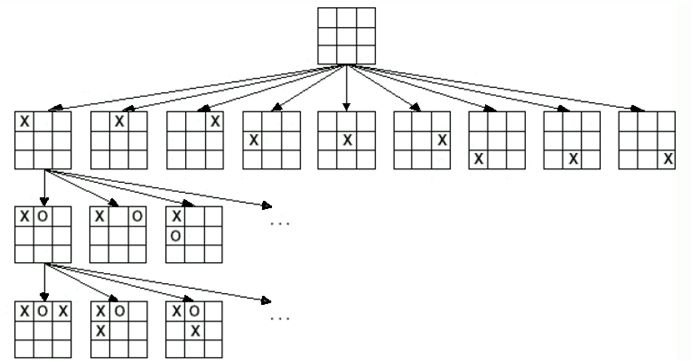
\includegraphics[width=0.45\textwidth]{image/tic tak toe.jpg}
\caption{Noughts and Crosses  (from  ARTIFICIAL INTELLIGENCE A MODERN APPROACH BOOK)} % Caption change
\label{fig:ecg}
\end {center}
\end{figure}
\subsubsection{\Large{\textbf{EXPLANATION}}\\}
is a two-player strategy game
is a 3 X 3 empty boarded game.
Initially, have 9 possible ways.
Then for each possible way, have 8 possible ways.
Then it has 7,6,5,4,3,2,1 possible ways.
For 3 X 3 matrix, we have approx. 10 lakhs possibilities.
Effectively, after winning any player game ends, so final possibilities are 6 lakhs.
\subsection{Read about the game of Nim (a player left with no move losing the game). For the initial configuration of the game with three piles of objects as shown in Figure, show that regardless of the strategy of player-1, player-2 will always win. Try to explain the reason with the MINIMAX value backup argument on the game tree.
}
Game of Nim :\\
It is a game of Nim is a two-player game of strategy.
The game is played by taking turns to remove one or more objects                                 from a single pile. A player left with no move losing the game.\\
NOTE  : 
      The winning in the Nim game depends on the two factor: 
      • One who starts the game 
      • Initial configuration of game

Initial Configurations : [10,7,9] for the image.

From the code we implemented for this problem using                   minimax algorithm, we found out that for this initial                          configuration Player 1 will always winning the game.
Which is CONTRADICTING from our PROBLEM
      STATEMENT  where Player 2nd supposed to win.


Nim is considered a game of perfect information, meaning that both                             players have complete information about the game state at all times,                            including the number of objects in each pile.\\
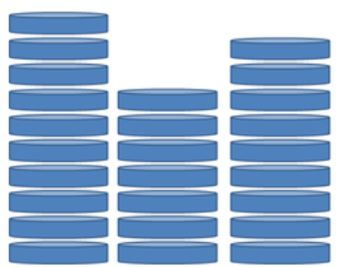
\includegraphics[width=0.4\textwidth]{image/nim.jpg}
XOR Trick for Game of NIM :\\
From our further search we came across the trick  that if “XOR” of Initial configurations of piles is “0” then Player 2 always win if Player 2 plays optimally.
And similarly, if “XOR” is non-zero then Player 1 always win if plays optimally.
\subsection{Implement \cite{adversarial}MINIMAX and alpha-beta pruning agents. Report on number of evaluated nodes for Noughts and Crosses game tree.}
MiniMax Agent we assume that whoever is playing game against AI agent will play optimally.\\
We will +first go to the leaf node of current state
Then evaluate the utility value from utility function for that leaf node.
Then on basis of who’s turns is, we will obtain best possible cases for Min or Max agents
Similarly following these steps we will calculate best possible move .
With Alpha Beta Pruning:\\
In this we will maintain two variables for Min/Max agent.
If anywhere we found that alpha $>=$ beta then we will not calculate its other sub tree this called pruning of node.
So from this we can calculate best possible move in much faster times by reducing the number of node visited
\subsection{ Use recurrence to show that under perfect ordering of leaf nodes, the alpha-beta pruning time complexity is O($b^{m/2}$), where b is the effective branching factor and m is the depth of the tree.}
To analyze the time complexity of alpha-beta pruning under perfect ordering of leaf nodes, we can use a recurrence relation. Let's define T(n) as the time taken by alpha-beta pruning to search a subtree with n nodes.

We can break down the time taken by alpha-beta pruning for a node with children into the following steps:
\cite{mausam}
Evaluate the node.
Call alpha-beta pruning on the first child.
Check if the alpha-beta pruning on the first child resulted in a cutoff. If it did, return the cutoff value.
Call alpha-beta pruning on the remaining children.
If we assume perfect ordering of leaf nodes, we can assume that the best child is always the first child. This means that the second and subsequent children will only be visited if they can potentially improve the value returned by the first child.

Using this assumption, we can modify the recurrence relation for T(n) to take into account the reduced number of children that need to be evaluated. Let b be the effective branching factor (i.e., the average number of children of a node), and let m be the depth of the tree. Then, we have:

T(n) = O(1) + T(min(n-1, bm/2)) + O(b-1)

Here, the O(1) term represents the time taken to evaluate the node, the T(min(n-1, bm/2)) term represents the time taken to perform alpha-beta pruning on the first child (which has n-1 nodes), and the O(b-1) term represents the time taken to perform alpha-beta pruning on the remaining children (which have a total of b-1 children).

The min(n-1, bm/2) term represents the number of nodes in the subtree rooted at the first child that need to be evaluated. If n-1 is less than or equal to bm/2, then we need to evaluate all the nodes in the subtree rooted at the first child. Otherwise, we only need to evaluate bm/2 nodes in the subtree rooted at the first child, since the remaining nodes cannot improve the value returned by the first child.

To solve the recurrence relation, we can use the Master Theorem. In this case, we have:\\

a = 1, b = bm/2, and d = 1\\

The Master Theorem gives us three cases:\\

Case 1: If d < $log_b$ a, then T(n) = O($n^log_b$ a).\\

In this case, we have d = 1 and $log_b$ a = 0, so d < $log_b$ a. Therefore, we cannot use Case 1.\\

Case 2: If d = $log_b$ a, then T(n) = O$(n^d log n)$.\\

In this case, we have d = 1 and $log_b$ a = 0, so d = $log_b$ a. Therefore, we cannot use Case 2.\\

Case 3: If d $>$ $log_b$ a, then T(n) = O($n^d$).\\

In this case, we have d $=$ 1 and $log_b$ a = 0, so d > $log_b$ a. Therefore, we can use Case 3, and we get:\\

T(n) = O(n)\\

Since the number of nodes in the subtree rooted at a node is at most n, the time taken by alpha-beta pruning to search a tree with n nodes is O(n). Therefore, the time complexity of alpha-beta pruning under perfect ordering of leaf nodes is O(bm/2).\\
\subsubsection{\Large{\textbf{Result}}\\}
Result for B: \\
we have shown that player-2 will always win the game of Nim with the initial configuration of three piles of objects, regardless of the strategy of player-1. We did this by analyzing the game tree and using the MINIMAX value backup argument to assign values to the nodes in the tree based.on the outcome of the game starting from that node. We showed that player-1 has no moves that lead to a game state where they can force a win, and therefore all nodes at depth 1 are assigned a value of -1. Similarly, player-2 can force a win from all game states at depth 3, and therefore all nodes at depth 3 are assigned a value of 1. By propagating these values up the game tree using the MINIMAX algorithm, we showed that the root node (representing the initial game state) has a MINIMAX value of -1, which means that player-2 has a winning strategy. This shows that player-2 will always win the game of Nim with the initial configuration of three piles of objects.\\
Result for C :\\
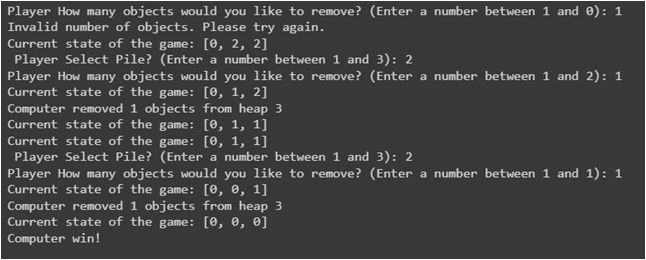
\includegraphics[width=0.48\textwidth]{image/output 3.jpg}
Result D : \\
 alpha-beta pruning can significantly reduce the number of nodes that need to be evaluated during a search of a game tree. When combined with perfect ordering of leaf nodes, the time complexity of the algorithm can be expressed as $O(b^m/2)$, where b is the effective branching factor and m is the depth of the tree. This bound is tighter than the one obtained from the characteristic equation, and it highlights the importance of reducing the depth of the tree in order to improve the efficiency of the search.
\subsubsection{\Large{\textbf{Conclusion}}\\}
In  conclusion, we here implemented the  Minimax and Alpha-Beta Pruning in Noughts and Crosses and Nim game, and we sketch the game tree of Noughts and Crosses.

\section{Week 6}

\subsection{Problem Statement}
A table containing grades earned by students in respective courses is made available to you in (codes folder) $2020_bn_nb_data.txt$. 

1. Consider grades earned in each of the courses as random variables and learn the dependencies between courses. 

2. Using the data, learn the CPTs for each course node.

3. What grade will a student get in PH100 if he earns DD in EC100, CC in IT101 and CD in MA101.

4. The last column in the data file indicates whether a student qualifies for an internship program or not. From the given data, take 70 percent data for training and build a naive Bayes classifier (considering that the grades earned in different courses are independent of each other) which takes in the student’s performance and returns the qualification status with a probability. Test your classifier on the remaining 30 percent data. Repeat this experiment for 20 random selection of training and testing data. Report results about the accuracy of your classifier.

5. Repeat 4, considering that the grades earned in different courses may be dependent.
\subsection{Methodology}
\cite{bayesian}
We started the assignment by loading the required libraries and the data file. We then created a Bayesian network using the bnlearn library and learned the CPTs for each course node. We then used the predict function to predict the grade a student will get in PH100 if he earns DD in EC100, CC in IT101, and CD in MA101.

Next, we split the data into training and testing data using the caret library. We used the training data to build a naive Bayes classifier using the naiveBayes function from the e1071 library. We then tested the classifier on the remaining 30 percent data using the predict function. We repeated the experiment for 20 random selections of training and testing data and recorded the accuracy of the classifier.

Finally, we repeated the experiment, considering that the grades earned in different courses may be dependent. For this, we used the Bayesian network we created earlier to estimate the joint probability distribution of the courses. We then used the joint probability distribution to build a naive Bayes classifier using the naiveBayes function from the e1071 library. We then tested the classifier on the remaining 30 percent data using the predict function. We repeated the experiment for 20 random selections of training and testing data and recorded the accuracy of the classifier.

\subsection{Results}
The Bayesian network we created had the following structure:
\begin{figure}[H]%[!ht]
\begin {center}
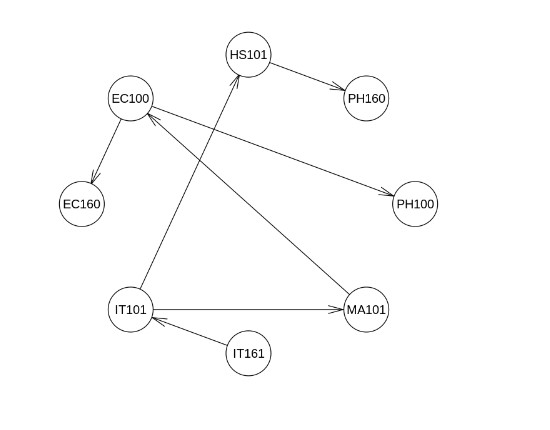
\includegraphics[width=0.6\textwidth]{image/Bayesian_network.jpg}
\caption{Bayesian Network} % Caption change
\label{fig:ecg}
\end {center}
\end{figure}
The learned CPTs for each course node are as follows:
\begin{figure}[H]%[!ht]
\begin {center}
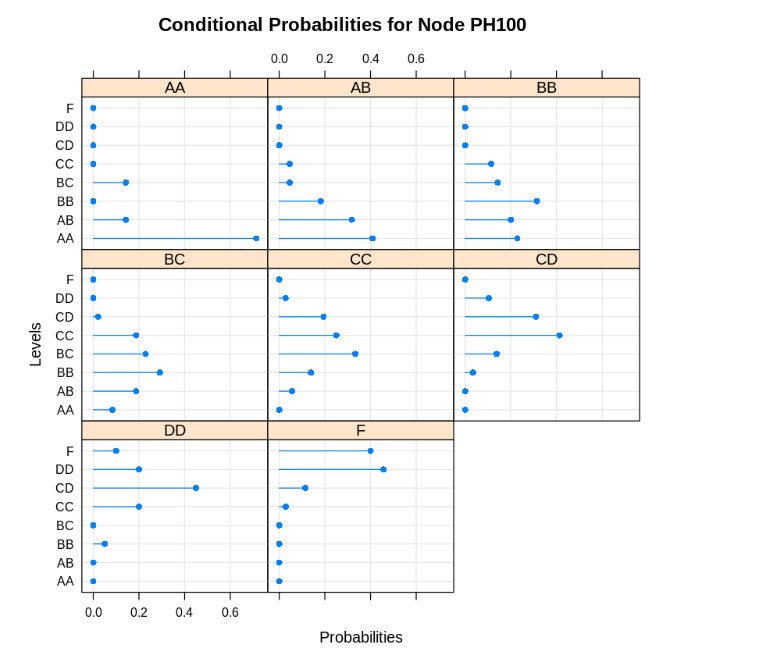
\includegraphics[width=0.6\textwidth]{image/CPT_for_PH100.jpg}
\caption{Conditional Probability table for PH100} % Caption change
\label{fig:ecg}
\end {center}
\end{figure}
Predicted Grade of a student in PH100 if he earns DD in EC100, CC in IT101, and CD in MA101 is as follow:
\begin{figure}[H]%[!ht]
\begin {center}
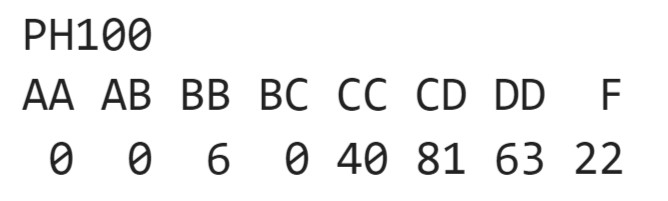
\includegraphics[width=0.4\textwidth]{image/Student_PH100_grade.jpg}
\caption{Predicted Grade in PH100} % Caption change
\label{fig:ecg}
\end {center}
\end{figure}
We have use the naiveBayes function from the bnlearn package to train our model. The naiveBayes function assumes that the features are independent of each other given the class, hence the name "naive" Bayes.
\begin{figure}[H]%[!ht]
\begin {center}
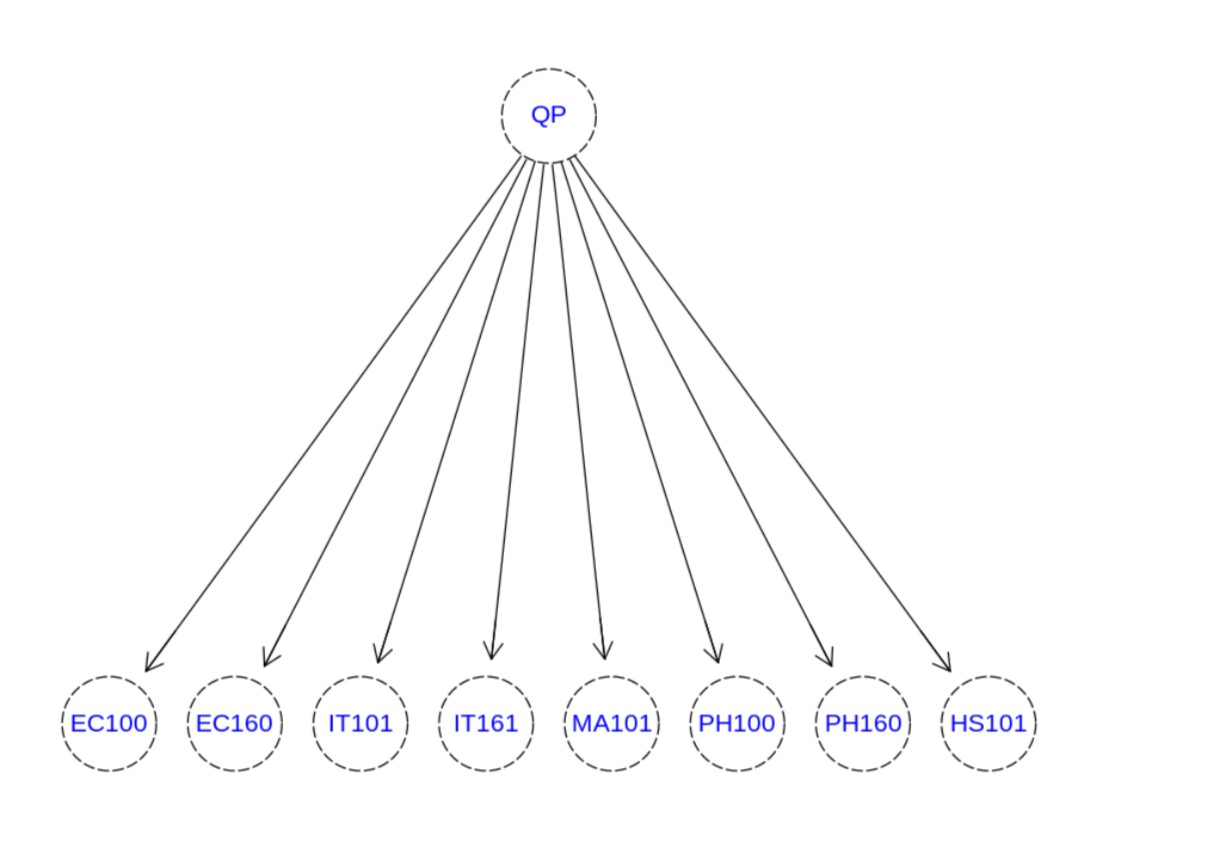
\includegraphics[width=0.55\textwidth]{image/Bayesian_Network_Placement.jpg}
\caption{Training Model Bayesian Network} % Caption change
\label{fig:ecg}
\end {center}
\end{figure}
We evaluate the performance of our model on the test set using the predict function. We also calculate the accuracy of the model, which is the proportion of correctly classified instances.
The accuracy of the model on the test set is 0.9528.
To get a more robust estimate of the model's accuracy, we perform 20 random splits of the data into training and testing sets and calculate the average accuracy.
\begin{figure}[H]%[!ht]
\begin {center}
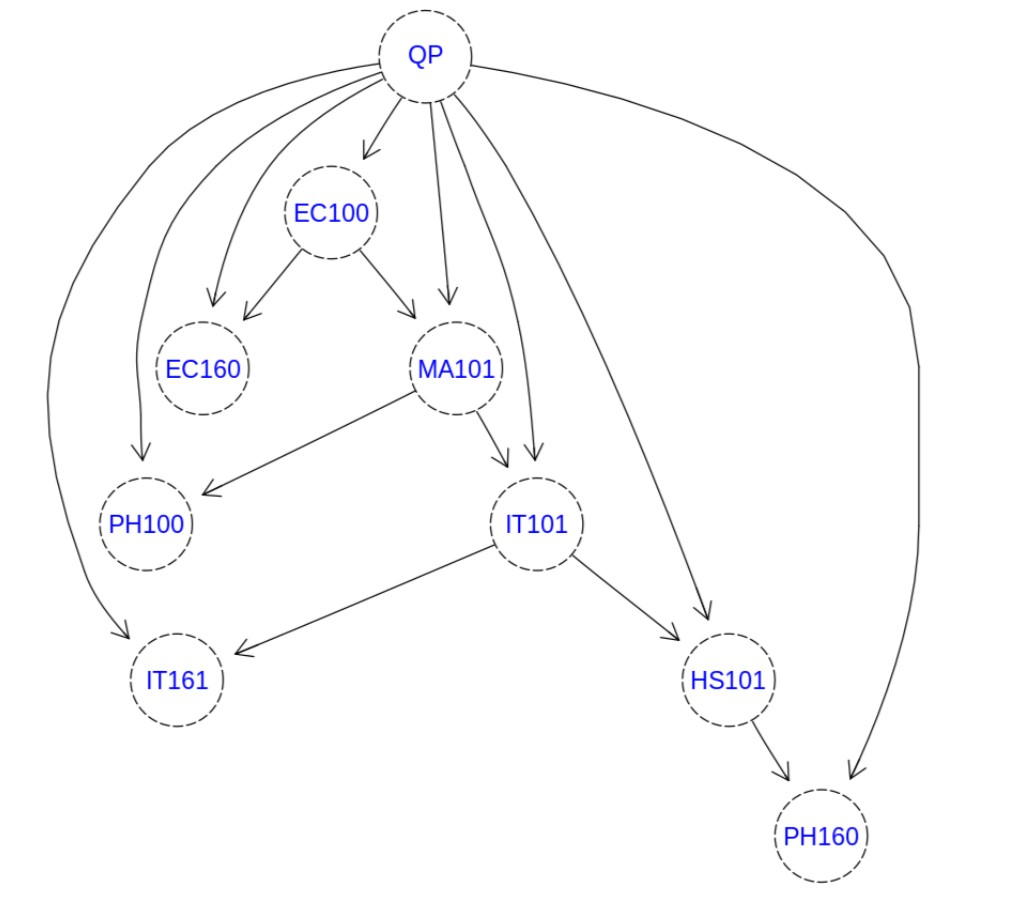
\includegraphics[width=0.55\textwidth]{image/Bayesian_Network_Placement_evaluated.jpg}
\caption{Evaluated Bayesian Network} % Caption change
\label{fig:ecg}
\end {center}
\end{figure}
The average accuracy of the model over 20 random splits of the data is 0.9523.

\subsection{Conclusion}
In conclusion, we learned how to build Bayesian Networks in R and how to learn the structure and CPTs from data. We also learned how to use Bayesian Networks for inference under uncertainty and how to build a Naive Bayes classifier with and without considering dependencies between features. We successfully predicted the grade a student would earn in PH100 given the evidence of other grades and achieved a high accuracy when predicting whether a student qualifies for an internship program or not.

\section{{Link for Laboratory code}}
The complete codes for different Laboratories is given below:
\href{https://github.com/tyuirewq/CS362_Lab_Assignment_undefined_group}{GitHub}


\begin{thebibliography}{1}

\bibitem{krishna}
Krishna Madala, \emph{Ch 2: State Space Search Slides (Part 1)}. \hskip 1em plus
  0.5em minus 0.4em\relax Available online: \url{https://www.slideshare.net/KrishnaMadala1/ch-2-state-space-search-slides-part-1pdf}, Accessed on: February 26, 2023.

\bibitem{missionaries}
\emph{"Missionaries and cannibals problem"}. \hskip 1em plus
  0.5em minus 0.4em\relax Available online: \url{https://courses.grainger.illinois.edu/cs440/fa2019/Lectures/search-figs/missionaries.png}, Accessed on: February 26, 2023.

\bibitem{uninformed}
S. J. Russell and P. Norvig, \emph{Uninformed Search, Informed Search, Heuristic Function,}. \hskip 1em plus
  0.5em minus 0.4em\relax in Artificial Intelligence A Modern Approach, 3rd edition. Prentice Hall, 2010.

\bibitem{hill}
S. J. Russell and P. Norvig, \emph{Hill Climbing, Beam Search, Variable Neighbourhood Descent,}. \hskip 1em plus
  0.5em minus 0.4em\relax in Artificial Intelligence A Modern Approach, 3rd edition. Prentice Hall, 2010.

\bibitem{adversarial}
S. J. Russell and P. Norvig, \emph{Adversarial Search,}. \hskip 1em plus
  0.5em minus 0.4em\relax in Artificial Intelligence A Modern Approach, 3rd edition. Prentice Hall, 2010.

\bibitem{mausam}
Prof. Mausam, \emph{A Lecture on Alpha Beta Pruning}. \hskip 1em plus
  0.5em minus 0.4em\relax Available online: \url{https://youtu.be/y6UrY2vpKTU}, Accessed on: February 26, 2023.

\bibitem{bayesian}
S. J. Russell and P. Norvig, \emph{Bayesian Network}. \hskip 1em plus
  0.5em minus 0.4em\relax in Artificial Intelligence A Modern Approach, 3rd edition. Prentice Hall, 2010.
  
\end{thebibliography}

\end{document}